\subsection{Гипербола}
 
\textsl{Гипербола} --- геометрическое место точек M Евклидовой плоскости, для которых абсолютное значение разности расстояний от $M$ до двух выделенных точек $F_1$ и $F_2$ (называемых фокусами) постоянно и равно удвоенной большой полуоси гиперболы.
\begin{equation}
\bigl||F_1M|-|F_2M|\bigr|=2a
\end{equation}
\textbf{Основные формулы для гиперболы:}
\begin{equation}
c^2=a^2+b^2
\end{equation}
Эксцентриситет гиперболы $e>1$ и вычисляется по формуле:
\begin{equation}
e=\frac{c}{a}
\end{equation}
Перецентрическое расстояние гиперболы вычисляется по следующей формуле:
\begin{equation}
q=a(e-1)
\end{equation}
Фокальный параметр вычисляется также, как и для эллипса:
\begin{equation}
p=\frac{b^2}{a}
\end{equation}
\textbf{Уравнение гиперболы:}

Канонический вид:
\begin{equation}
\frac{x^2}{a^2}-\frac{y^2}{b^2}=1
\end{equation}
\begin{figure}[h!]
\centering
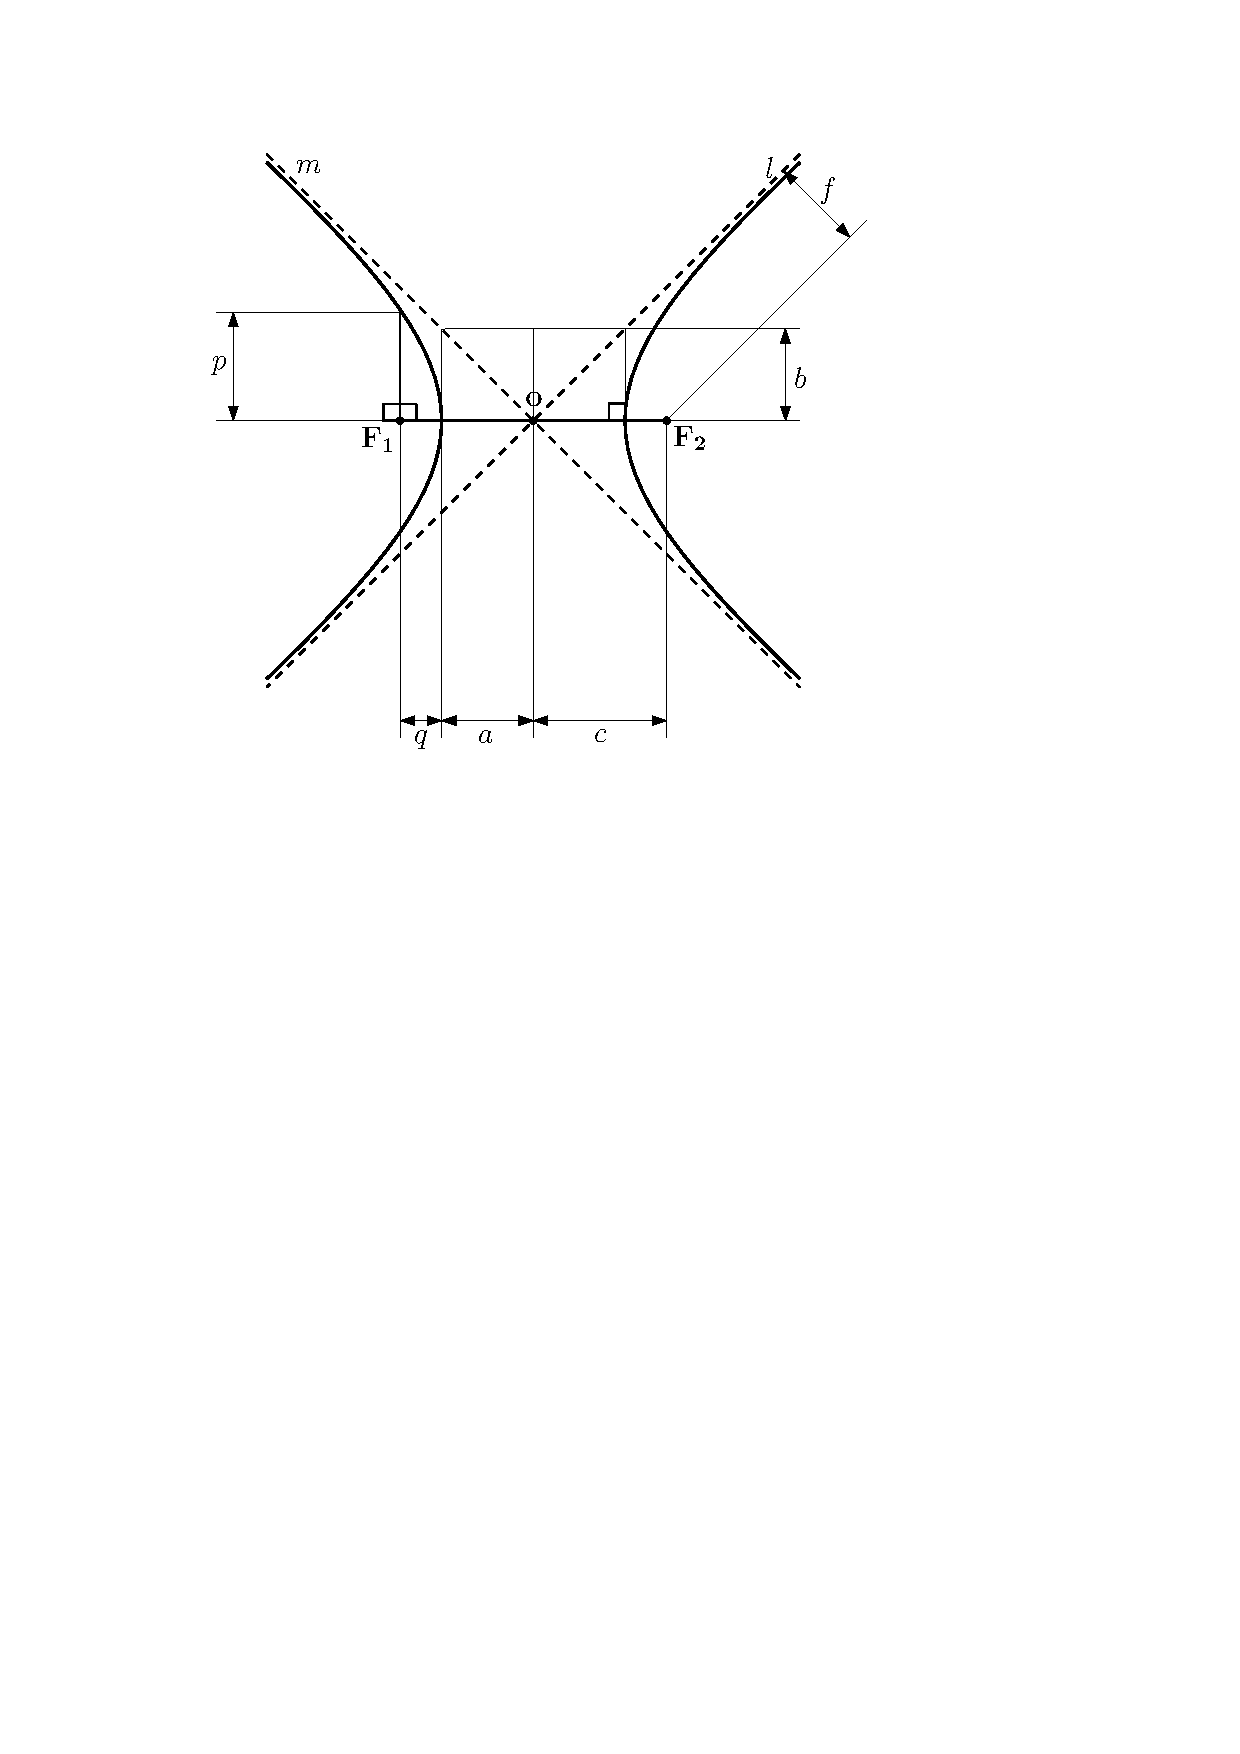
\includegraphics[width = 0.7\textwidth]{Hiperbola}
\caption{Гипербола \label{pic:the-pic}}
\end{figure}